\documentclass[a4paper]{article}
\usepackage[utf8]{inputenc}
\usepackage[russian,english]{babel}
\usepackage[T2A]{fontenc}
\usepackage[left=10mm, top=20mm, right=18mm, bottom=15mm, footskip=10mm]{geometry}
\usepackage{indentfirst}
\usepackage{amsmath,amssymb}
\usepackage[italicdiff]{physics}
\usepackage{graphicx}
\graphicspath{{images/}}
\DeclareGraphicsExtensions{.pdf,.png,.jpg}
\usepackage{wrapfig}
\usepackage{pgfplots}

\usepackage{caption}
\captionsetup[figure]{name=Рисунок}
\captionsetup[table]{name=Таблица}


\title{\underline{Лабораторная работы 2.4.1}}
\author{Старостин Александр, Б01-401}
\date {28 Февраля, 2025 год}


\begin{document}

\maketitle
\newpage

\textbf{Определение теплоты испарения жидкости}

\section{Аннотация}
    \par \textbf{Цель работы:} 1) измерение давления насыщенного пара жидкости при разной температуре; 2) вычисление по полученным данным теплоты испарения с помощью уравнения Клайперона-Клаузиса. \\

    \par \textbf{В работе используются:} термостат; герметический сосуд, заполненный исследуемой жидкостью; отсечённый микроскоп.

\section{Теоретические сведения}

Теплоту испарения жидкости можно определить из формулы Клайперона-Клаузиса (описание кривой фазового перехода):

\begin{equation}
	\frac{dP}{dT} = \frac{L}{T(V_2 - V_1)},
\end{equation}

где $P$ - давление насыщенного пара жидкости при абсолютной температуре жидкости $T$, $L$ - теплота парообразования, $V_2$ - объём пара, $V_1$ - объём жидкости. \\

В формуле (1) $L$, $V_1$, и $V_2$ должны относиться к одному и тому же количеству вещества. В нашем случае к 1 молю.   \\


При нашей точности опыта $V_1$ в (1) можно пренебречь и $V_2 = V$ \\

Уравнение Вандер-Ваальса:

\begin{equation}
	(P + \frac{a}{V^2})(V-b) = RT.
\end{equation}


Коэффициентами $a$ и $b$ можно пренебречь, тк $b$ одно порядка с $V_1$, а $a$ при давлении ниже атмосферного вносит малую ошибки (при пренебрежении). \\

Получаем, что:

\begin{equation}
	V = \frac{RT}{P}.
\end{equation}

Подставляя (3) в (1), пренебрегая $V_1$ и выражая $L$, получаем:

\begin{equation}
	L = \frac{RT^2}{P} \frac{dP}{dT} = -R \frac{d(ln P)}{d(1/T)}.
\end{equation}

Используя (1) и (4) и найдя отношения через графики, можно найти значение $L$

\section{Установка}

Схема установки:

\begin{figure}[ht]
        \center{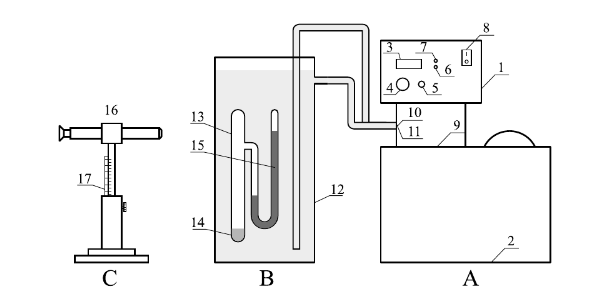
\includegraphics[scale=0.5]{stand}}
        \caption{Схема установки для определения теплоты испарения.}
        \label{ustanovka}
    \end{figure}

В запаянной трубке 13 находится исследуемая жидкость 14 (в нашем случае спирт). В сосуде B находится вода. Меняя температуру воды с помощью термостата A (температура не должны превышать $40 ^\circ C$, тк при такой температуре в наших условиях спирт начнёт закипать), мы будем менять давление насыщенного пара в колбе 13 (увеличивая $T$, мы будем увеличивать $P_\text{нас}$). И по разнице высот столбиков на манометре 15 мы смодем измерить $P_\text{нас}$. Сделать это можно при помощи микроскопа 16 (по нему будем определять границы столбцов) и электронного измерительного прибора 17 (он будет фиксировать длину сдвига микроскопа, а следовательно, и мерить разницу высот).

\section{Ход работы}

\subsection{Измерение начальных условий}

В начальный момоент времени:\\

$\Delta H = |H_2 - H_1| = (44.45 \pm 0.03 * \sqrt{2})\text{ мм} \approx (44.45 \pm 0.04)\text{ мм}$,

$\sigma_{\Delta H} = 0.04\text{ мм}$, \\

$t_0 = (20.21 \pm 0.03)^\circ C$,

$\sigma_t = 0.03^\circ C$,

$\sigma_T = 0.03 K$, \\

Вещество в колбе - спирт,\\

$R = (8.31 \pm 0.01) \frac{\text{Дж}}{\text{К*моль}}$,

$\sigma_R = 0.01 \frac{\text{Дж}}{\text{К*моль}}$, \\

$g = (9.8 \pm 0.1) \frac{\text{м}}{\text{с}^2}$,

$\sigma_g = 0.1\frac{\text{м}}{\text{с}^2}$, \\

$\rho_\text{рт} = (13595.1 \pm 0.1) \frac{\text{кг}}{\text{м}^3}$,

$\sigma_{\rho_\text{рт}} = 0.1 \frac{\text{кг}}{\text{м}^3}$, \\

$P = P_\text{нас} = \rho_\text{рт}g \Delta H$,

$\sigma_P = P \sqrt{(\frac{\sigma_{\Delta H}}{\Delta H})^2 + (\frac{\sigma_g}{g})^2 + (\frac{\sigma_{\rho_\text{рт}}}{\rho_\text{рт}})^2}$. \\

\subsection{Измерения при нагревании}

Проведём измерения при нагревании:

\begin{table}[h!]
    \centering
    \begin{tabular}{|c|c|c|c|c|c|c|}
    \hline
       $t ^\circ C$  & $T\text{, K}$ & $H \text{, мм}$ & $P\text{, Па}$ & $1/T$ \text{, 1/K} & $ln P$  & $L\text{, Дж/моль}$  \\ \hline

    24.00 & 297.15 &   54.7 & 7287.8  & 0.003365 & 8.89  & 54368.9 \\ \hline
    25.00 & 298.15 &   57.5 & 7660.8  & 0.003354 & 8.94  & 52070.1 \\ \hline
    26.00 & 299.15 &   60.7 & 8083.2  & 0.003343 & 9.00  & 49681.0 \\ \hline
    27.00 & 300.15 &   64.5 & 8593.5  & 0.003332 & 9.06  & 47043.9 \\ \hline
    28.00 & 301.15 &   69.7 & 9280.9  & 0.003320 & 9.14  & 43849.9 \\ \hline
    29.00 & 302.15 &   73.1 & 9736.6  & 0.003310 & 9.18  & 42075.9 \\ \hline
    30.00 & 303.15 &   77.1 & 10277.5 & 0.003299 & 9.24  & 40125.6 \\ \hline
    31.00 & 304.15 &   81.2 & 10822.4 & 0.003288 & 9.29  & 38357.1 \\ \hline
    32.00 & 305.15 &   85.7 & 11423.3 & 0.003277 & 9.34  & 36578.8 \\ \hline
    33.00 & 306.15 &   90.0 & 11990.9 & 0.003266 & 9.39  & 35076.2 \\ \hline
    34.00 & 307.15 &   95.4 & 12713.0 & 0.003256 & 9.45  & 33300.3 \\ \hline
    35.00 & 308.15 &  100.7 & 13417.8 & 0.003245 & 9.50  & 31756.9 \\ \hline

    \end{tabular}
    \caption{измерения при нагревании}
    \end{table}

$L$ в каждой ситуации вычислялось по левой части формулы (4) уже после определения отношения $\frac{dP}{dT}$ по графику $P$ от $T$.

\subsection{Измерения при охлаждении}

Проведём измерения при охлаждении:

\newpage

\begin{table}[h!]
    \centering
    \begin{tabular}{|c|c|c|c|c|c|c|}
    \hline
       $t ^\circ C$  & $T\text{, K}$ & $H \text{, мм}$ & $P\text{, Па}$ & $1/T$ \text{, 1/K} & $ln P$  & $L\text{, Дж/моль}$  \\ \hline

    35.00 & 308.15 &  100.7 & 13417.8 & 0.003245 & 9.50  & 31756.9 \\ \hline
    34.00 & 307.15 &   96.0 & 12786.3 & 0.003256 & 9.46  & 33109.4 \\ \hline
    33.00 & 306.15 &   91.1 & 12130.8 & 0.003266 & 9.40  & 34671.7 \\ \hline
    32.00 & 305.15 &   87.0 & 11588.5 & 0.003277 & 9.36  & 36057.3 \\ \hline
    31.00 & 304.15 &   81.5 & 10854.4 & 0.003288 & 9.29  & 38244.1 \\ \hline
    30.00 & 303.15 &   77.8 & 10366.8 & 0.003299 & 9.25  & 39780.1 \\ \hline
    29.00 & 302.15 &   73.1 & 9739.3  & 0.003310 & 9.18  & 42064.3 \\ \hline
    28.00 & 301.15 &   68.7 & 9158.4  & 0.003320 & 9.12  & 44436.8 \\ \hline
    27.00 & 300.15 &   65.2 & 8689.4  & 0.003332 & 9.07  & 46524.6 \\ \hline
    26.00 & 299.15 &   62.9 & 8377.6  & 0.003343 & 9.03  & 47934.9 \\ \hline
    25.00 & 298.15 &   59.4 & 7911.3  & 0.003354 & 8.98  & 50421.5 \\ \hline
    24.00 & 297.15 &   57.1 & 7600.9  & 0.003365 & 8.94  & 52129.3 \\ \hline

    \end{tabular}
    \caption{измерения при охлаждении}
    \end{table}

$L$ в каждой ситуации вычислялось по левой части формулы (4) уже после определения отношения $\frac{dP}{dT}$ по графику $P$ от $T$.

\subsection{Построение графиков}

\subsubsection{График $P$ от $T$}
Построим график зависимости $P$ от $T$ для левой части формулы (4):

\begin{figure}[ht]
        \center{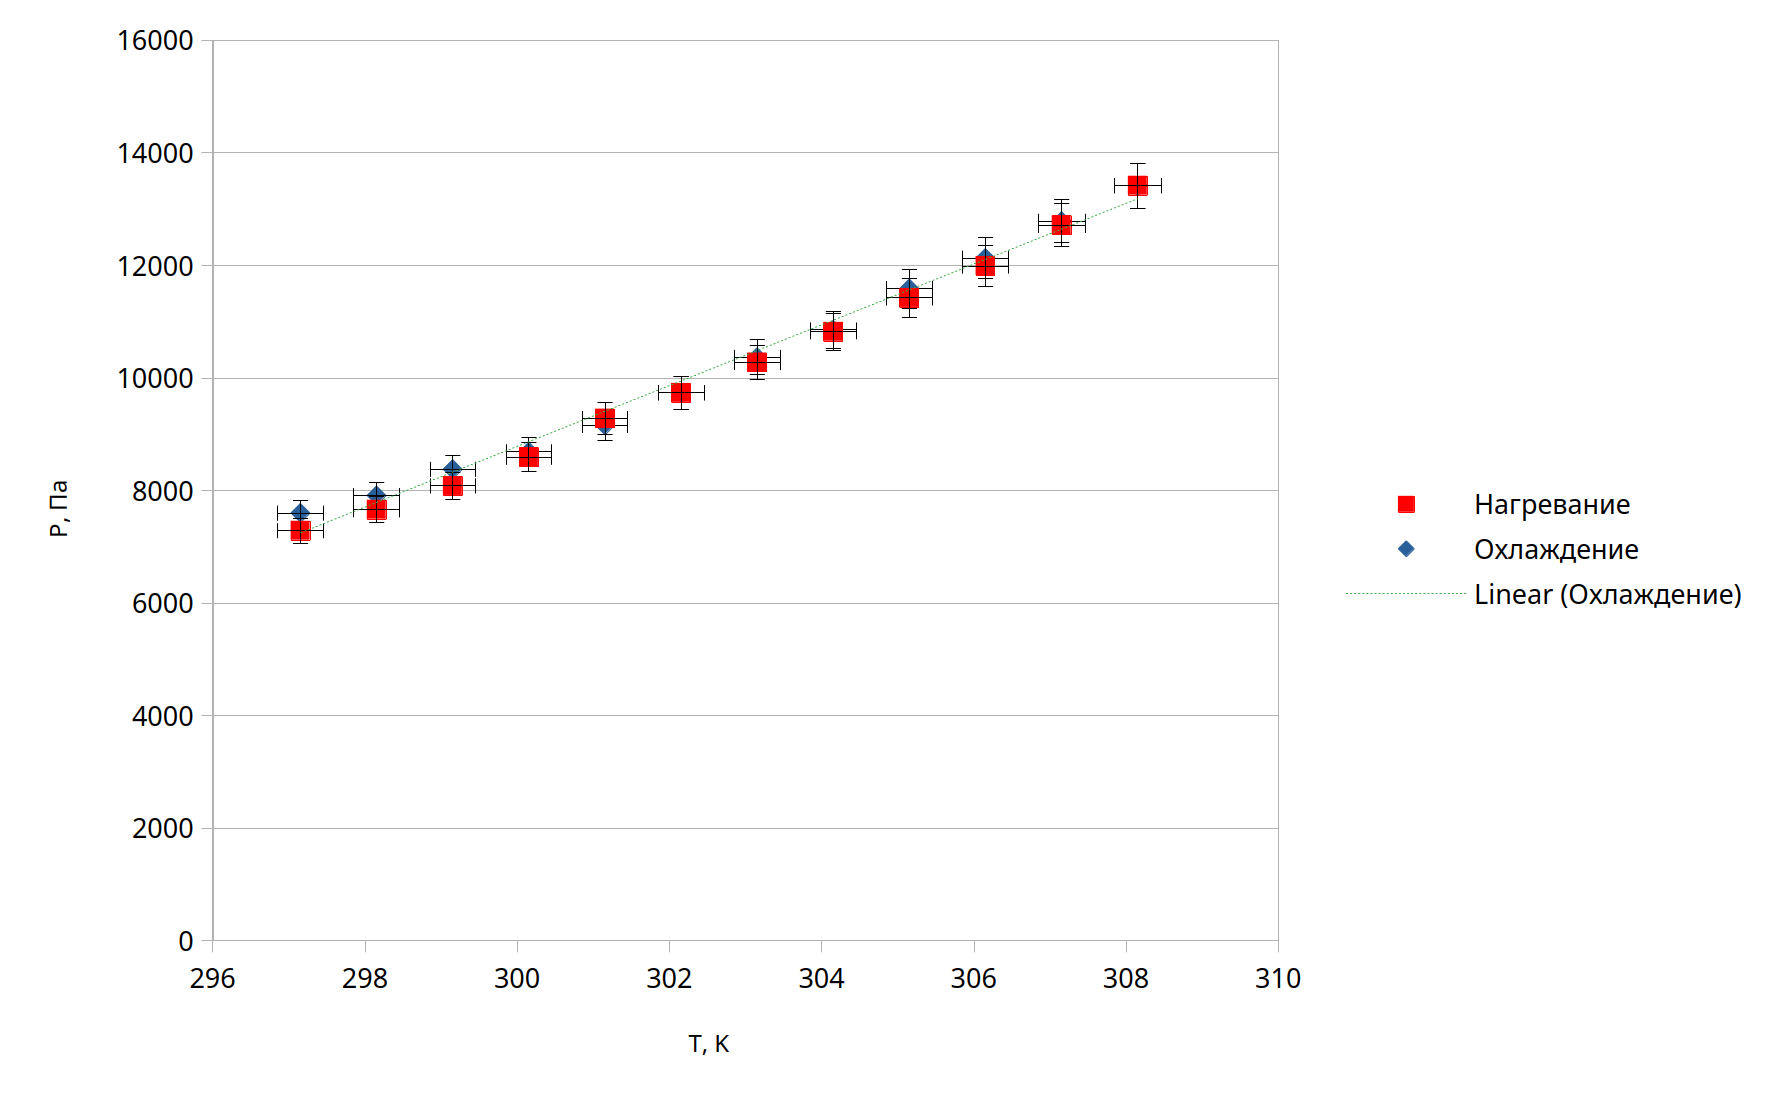
\includegraphics[scale=0.32]{chart_P_T}
        \caption{График зависимости $P$ от $T$.}
        \label{ustanovka}
    \end{figure}

Проведём наилучшую прямую $f(x) = kx + b$ по МНК.\\

Тогда $k = \frac{dP}{dT} = \frac{<xy> - <x><y>}{<x^2> - <x>^2} = 539.66 \text{ Па/K}$.\\

И $\sigma_k = \sqrt{\frac{1}{24}} \sqrt{\frac{<y^2> - <y>^2}{<x^2> - <x>^2} - k^2} = 10.79 \text{ Па/K}$.\\

Тогда $\frac{dP}{dT} = (540 \pm 11) \text{ Па/K}$. Используя это отношение и формулу (4), можно вычислить $L$ в каждой точке. Результаты вычислений приведены в таблицах (1) и (2).\\

При этом в каждом случае: $\sigma_L = L \sqrt{(\frac{\sigma_k}{k})^2 + (\frac{\sigma_R}{R})^2 + (\frac{\sigma_P}{P})^2 + (2 \frac{\sigma_T}{T})^2}$\\

\subsubsection{График $lnP$ от $1/T$}
Построим график зависимости $lnP$ от $1/T$ для правой части формулы (4):

\begin{figure}[ht]
        \center{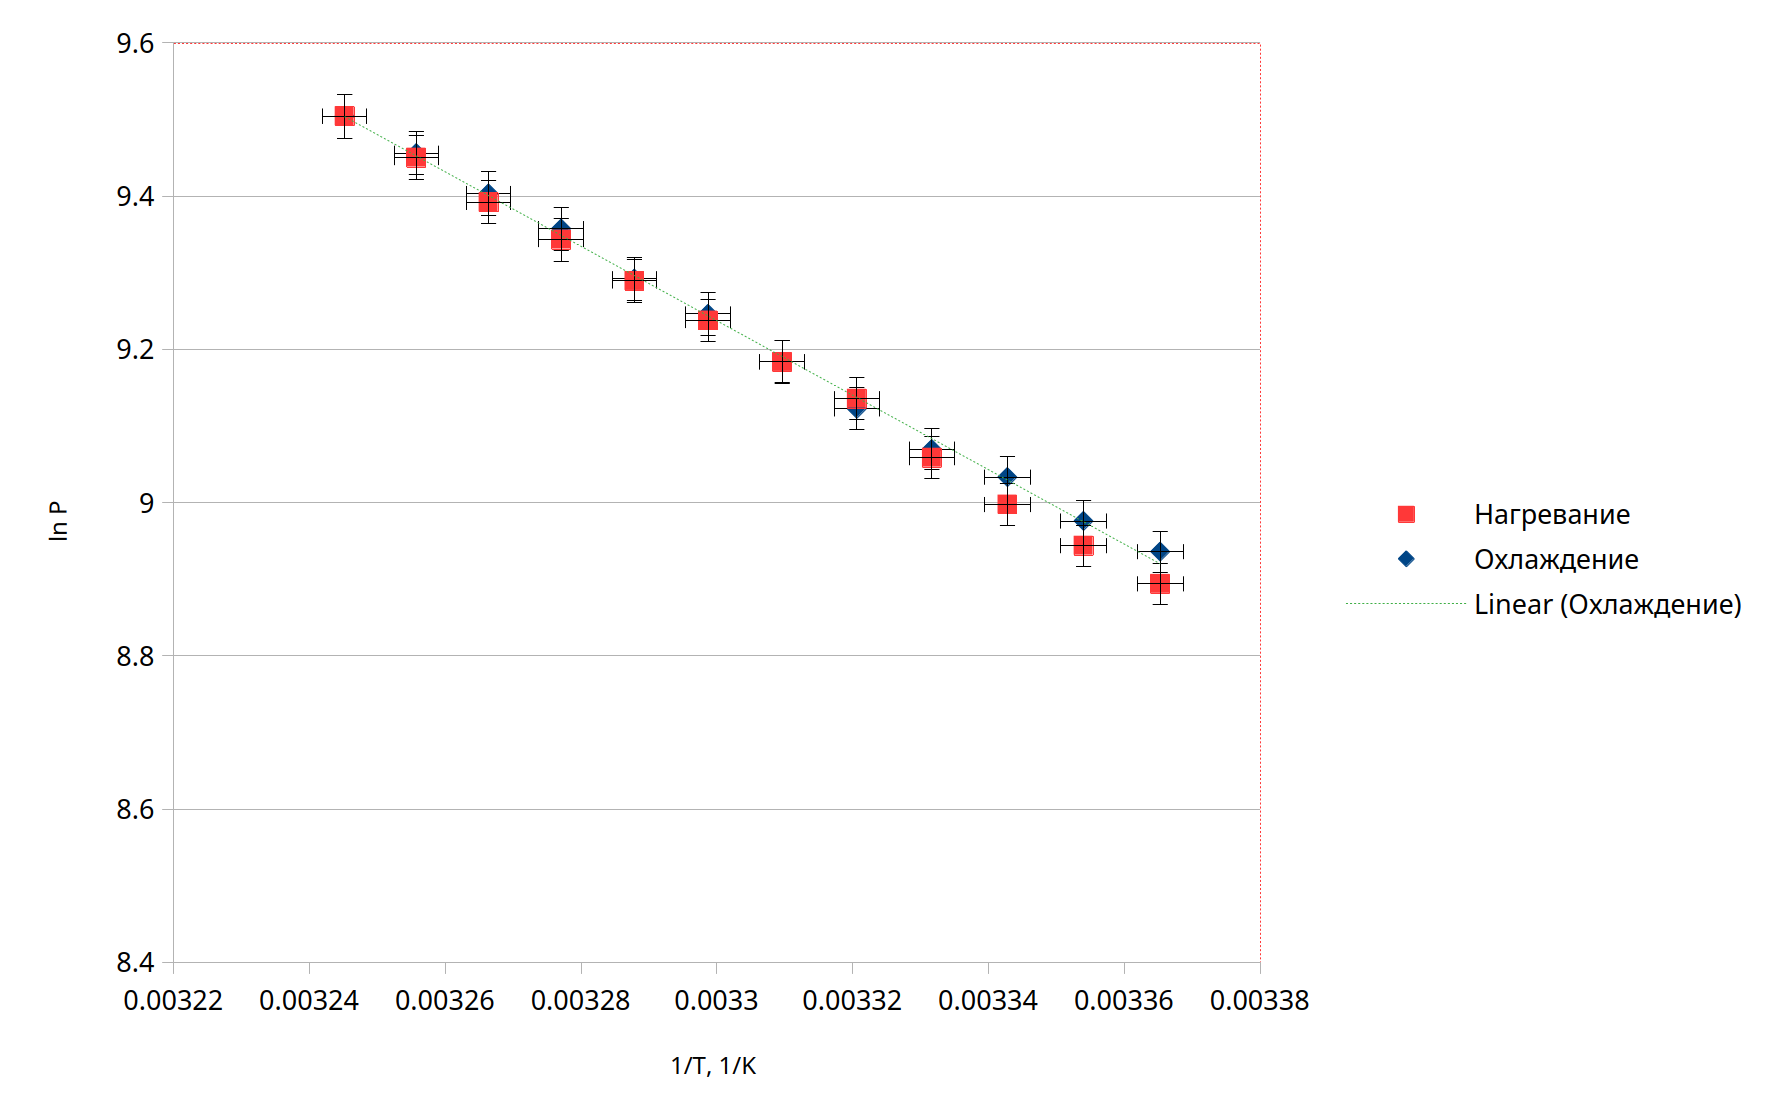
\includegraphics[scale=0.32]{chart_lnP_1⁄T}
        \caption{График зависимости $lnP$ от $1/T$.}
        \label{ustanovka}
    \end{figure}

Проведём наилучшую прямую $f(x) = kx + b$ по МНК.\\

Тогда $k = \frac{d(lnP)}{d(1/T)} = \frac{<xy> - <x><y>}{<x^2> - <x>^2} = -4857.7 \text{ K}$.\\

И $\sigma_k = \sqrt{\frac{1}{24}} \sqrt{\frac{<y^2> - <y>^2}{<x^2> - <x>^2} - k^2} = 97.15 \text{ K}$.\\

Тогда $\frac{d(lnP)}{d(1/T)} = (-4858 \pm 97) \text{ K}$. Используя это отношение и формулу (4), можно вычислить среднюю $L$ в этом диапозоне температур.\\

Тогда $L = 40369.98 \text{ Дж/моль}$.\\

При этом $\sigma_L = L \sqrt{(\frac{\sigma_k}{k})^2 + (\frac{\sigma_R}{R})^2} = 807.53 \text{ K}$\\

Получаем, что $L = (40370 \pm 808)\text{ Дж/моль}$.\\

\subsection{Вывод}

Мы вычислили $L$ двумя способами: в каждой точке и среднюю в диапозоне температур. Оба результата находятся в согласии друг с другом. Результаты измерений приблизительно совпадают с табличными ($L_\text{таб} =40700 \text{ Дж/моль}$).

\end{document}





